\chapter{Metodología}
\label{cap:metodologia}

Este capítulo expone cómo se construyó el algoritmo propuesto y cómo se lo evaluó. Después del enfoque
y las variables del estudio, la Sección~\ref{sec:corpus} presenta los conjuntos de imágenes. La
Sección~\ref{sec:propuesta} define el algoritmo y los métodos comparativos, y la
Sección~\ref{sec:ajuste} describe el ajuste de su radio y su peso. Siguen la evaluación de la calidad
(Sección~\ref{sec:protocolo-calidad}), la de la aplicación a la detección
(Sección~\ref{sec:protocolo-deteccion}) y el examen de la hipótesis
(Sección~\ref{sec:examen-hipotesis}). La Figura~\ref{fig:metodologia} reúne esas etapas en un diagrama.
En él, los dos conjuntos de imágenes reciben el mismo preprocesamiento y se fusionan con los mismos siete
métodos. A partir de ahí el diagrama se abre: la rama izquierda lleva a la evaluación de la calidad, con
el conjunto TNO, y la derecha, a la de la detección, con el conjunto M3FD. Las dos ramas terminan en el
examen de la hipótesis. La flecha doble indica que el enjambre evalúa el propio algoritmo y le devuelve
el radio y el peso.

\begin{figure}[htbp]
\centering
\caption{Etapas del estudio}
\label{fig:metodologia}
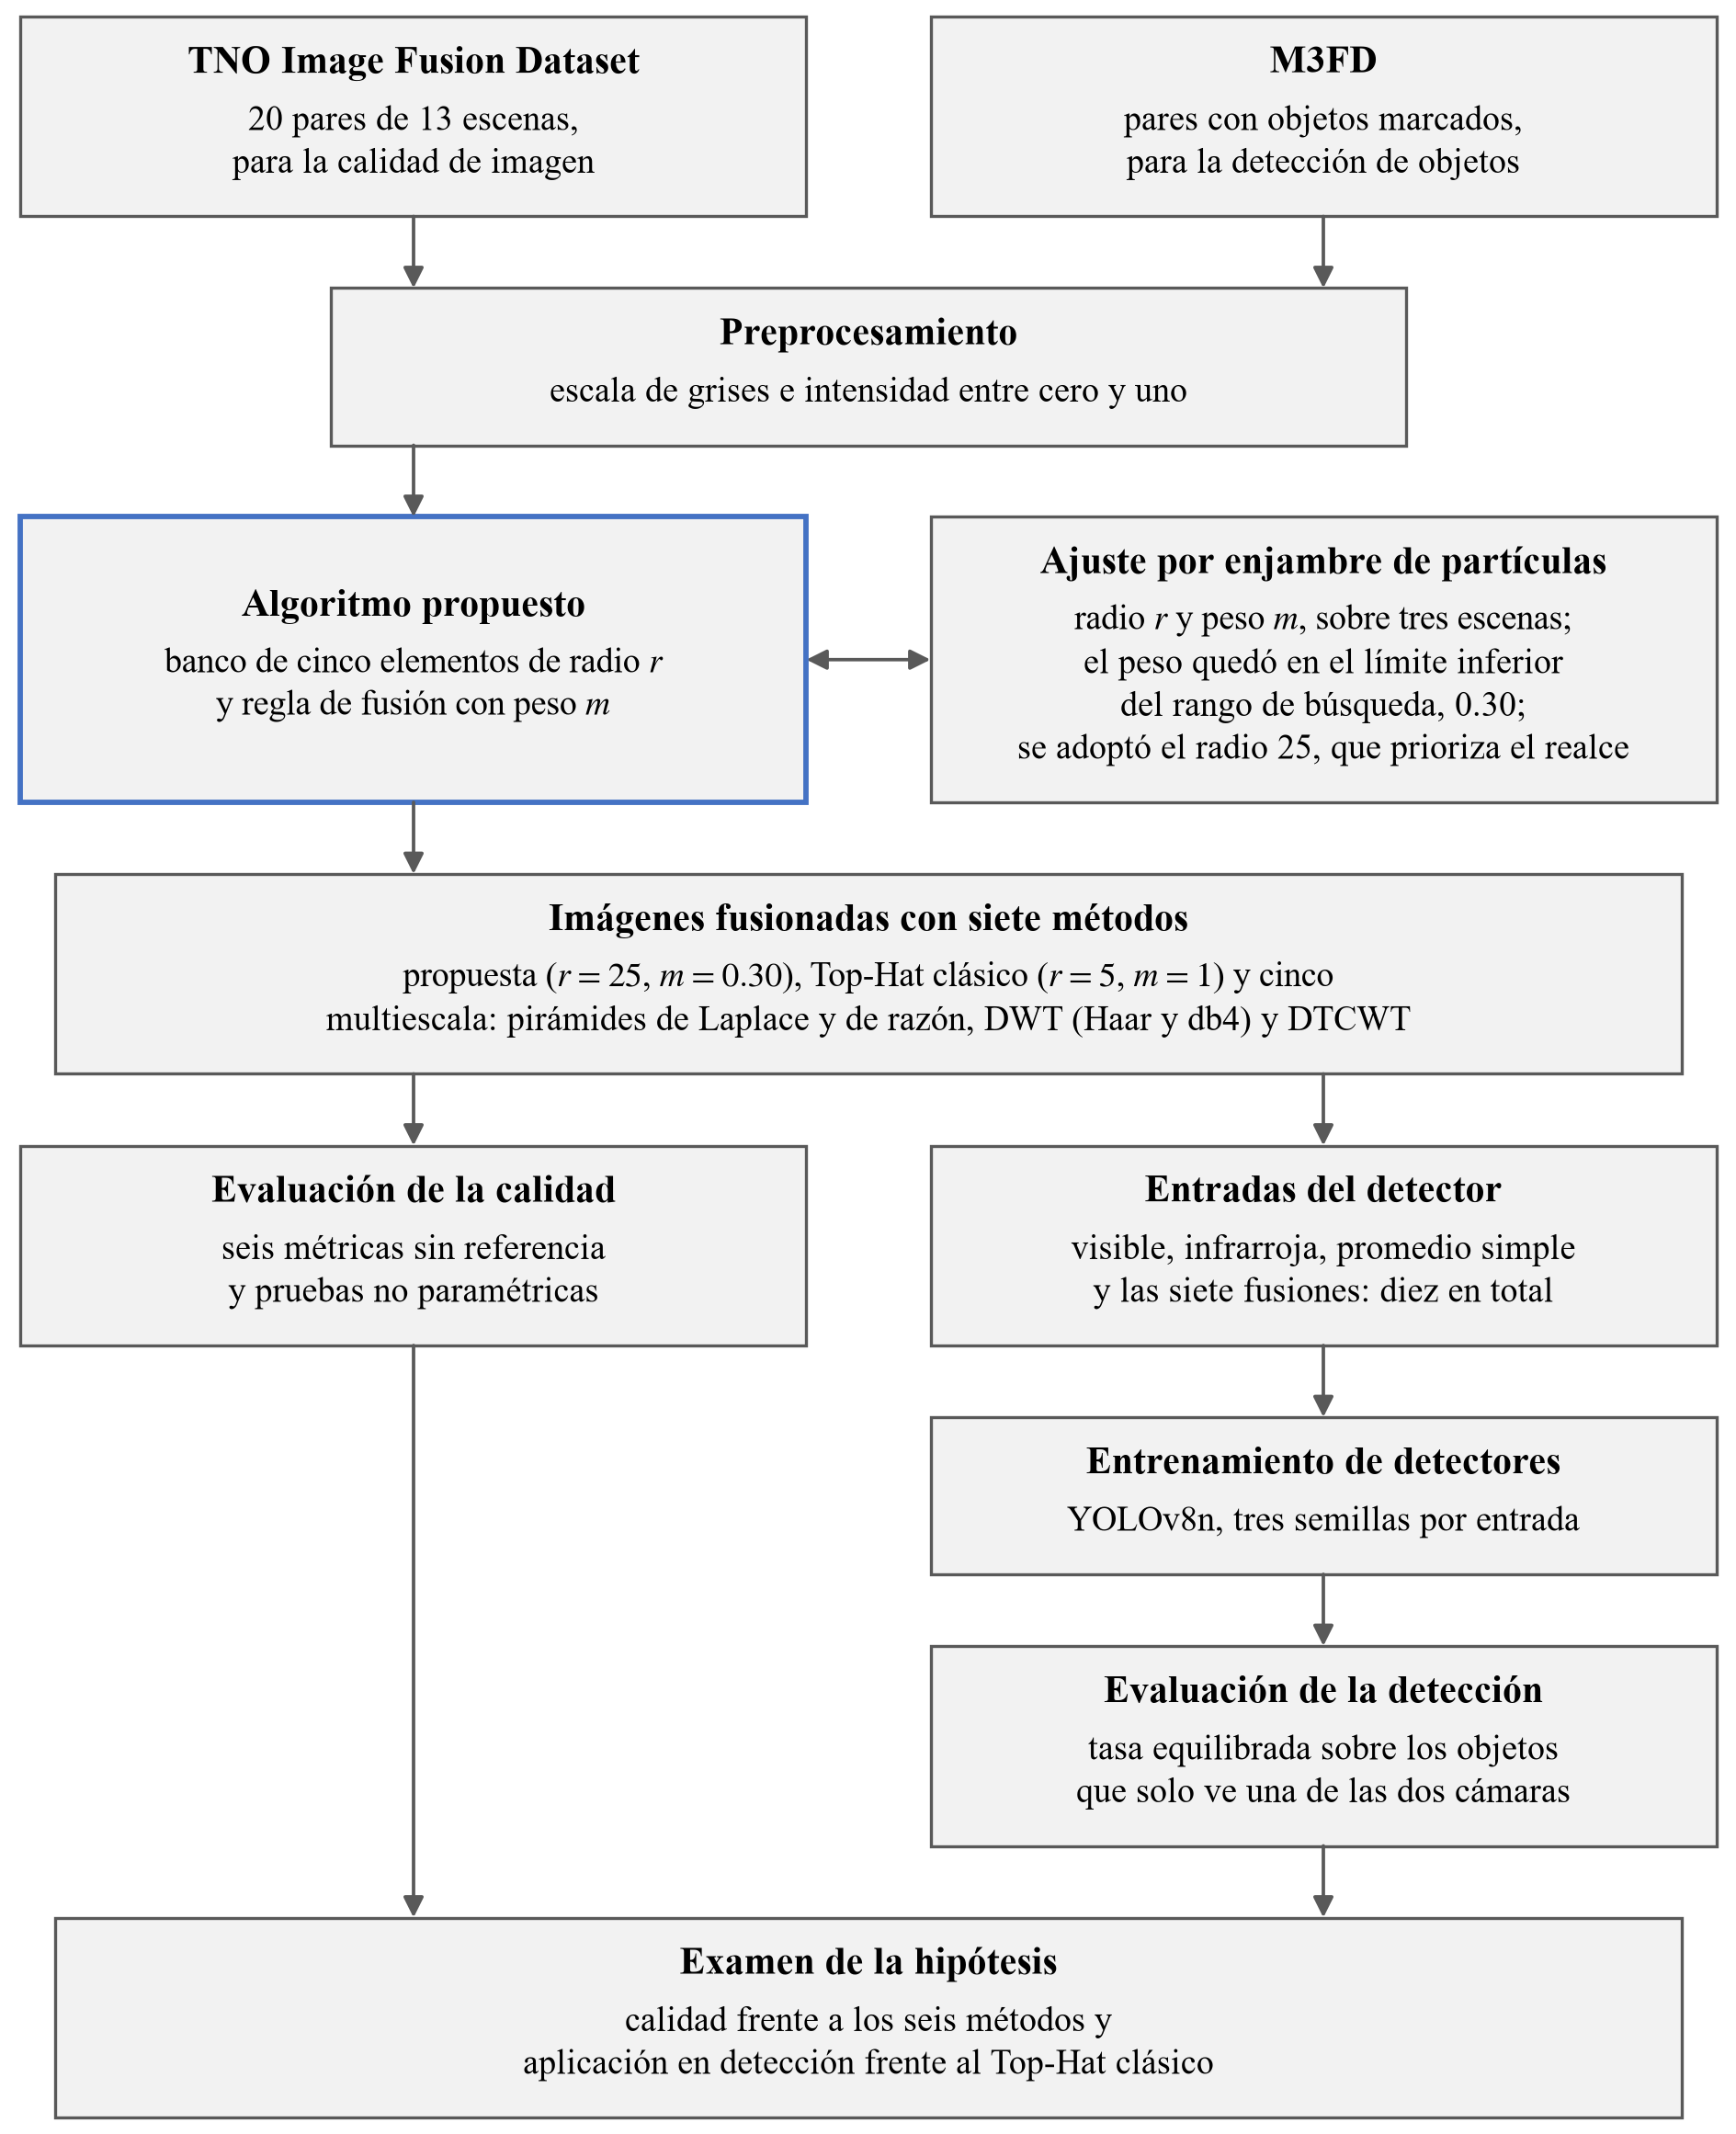
\includegraphics[width=\textwidth]{figuras/fig_metodologia}
\nota{Elaboración propia. El recuadro azul destaca el algoritmo propuesto.}
\end{figure}

El enfoque fue cuantitativo. Cada conclusión se apoyó en mediciones numéricas sobre conjuntos fijos de
imágenes, analizadas con pruebas estadísticas o, donde no hubo una prueba propia, de forma descriptiva, y no en el juicio de observadores. El diseño fue
experimental y comparativo. Todos los métodos procesaron las mismas imágenes y se midieron con el mismo
procedimiento, de modo que de una condición a otra solo varió la forma de fusionar.

La evaluación se hizo en dos planos. El primero es la calidad de la imagen fusionada, juzgada por sí
misma con métricas numéricas. El segundo es su aplicación, es decir, cuánto le sirve esa imagen a un
detector automático de objetos. Cada plano usa su propio conjunto de imágenes y se informa por
separado, porque un método puede destacar en uno y no en el otro.

Las variables del estudio fueron las siguientes:
\begin{itemize}
\item \textbf{Variable independiente:} El método de fusión. En la evaluación de calidad tomó siete
valores: el algoritmo propuesto, el Top-Hat clásico y cinco métodos multiescala. En la detección hubo
diez entradas para el detector: la imagen visible, la infrarroja, el promedio simple de ambas y las
siete fusiones.
\item \textbf{Variables dependientes:} Las seis métricas de calidad de imagen y la tasa de acierto
equilibrada del detector sobre los objetos vistos por una sola cámara.
\item \textbf{Variables controladas:} En la calidad, los pares de imágenes, el preprocesamiento y el
cálculo de las métricas. En la detección, los cuadros, las etiquetas de los objetos y la configuración
del detector.
\end{itemize}

\section{Conjuntos de imágenes y preprocesamiento}
\label{sec:corpus}

La calidad de imagen se midió sobre el \textit{TNO Image Fusion Dataset} \parencite{toet2014, toet2017}. El
conjunto reúne pares de imágenes nocturnas de escenas militares y de vigilancia, captados a la vez por una cámara
visible y por una térmica. En buena parte de los pares, la visible proviene de una cámara con
intensificador de imagen, que amplifica la escasa luz nocturna. El TNO es el conjunto público más usado
en la fusión visible-infrarroja \parencite{liu2022}, lo que facilita situar los resultados junto a los de
otros trabajos.

Los pares vienen registrados por sus autores: las dos imágenes de cada par cubren la misma escena desde
el mismo punto de vista. Aun así, en algunos se advierte un corrimiento vertical de varios píxeles entre
ambas. Ese corrimiento no se corrigió, para trabajar con el conjunto tal como se distribuye, y tampoco
se midió su efecto.

Se trabajó con veinte pares, que corresponden a trece escenas. Cuatro de esas escenas aportan más de una
toma, en otro instante o desde otro ángulo, y entre ellas reúnen once pares. La distinción tiene peso en
la estadística, porque dos tomas de una misma escena no son observaciones del todo independientes. La
Sección~\ref{sec:protocolo-calidad} explica cómo se tuvo en cuenta esa dependencia. También se comprobó
que en ningún par la imagen visible fuera una copia de la infrarroja.

El preprocesamiento se limitó a lo indispensable. Cada imagen se convirtió a escala de grises y sus
niveles se llevaron al intervalo de cero a uno con la Ecuación~\eqref{eq:intensidad}. No se aplicó
ningún realce, filtrado ni corrección de contraste previos, porque su efecto se habría confundido con el
del método de fusión.

La aplicación a la detección se evaluó sobre M3FD \parencite{liu2022}, un conjunto de 4200 pares
visible-infrarrojo registrados. Cada objeto está marcado con una caja y pertenece a una de seis clases:
personas, autos, autobuses, motocicletas, luces y camiones. Las escenas, urbanas y naturales, se tomaron
de día y de noche. Este conjunto se usó solo para la detección. Se le aplicó el mismo preprocesamiento
que al TNO, y por eso el detector recibió la imagen visible en escala de grises. Las imágenes de todas las entradas del detector
se guardaron en formato JPEG (del inglés \textit{Joint Photographic Experts Group}) de 8 bits. La
Sección~\ref{sec:det-datos} describe cómo se repartieron sus cuadros.

\section{El algoritmo de fusión propuesto}
\label{sec:propuesta}

El algoritmo propuesto es un operador Top-Hat de una sola escala: todos sus elementos estructurantes
comparten un mismo tamaño. Para fusionar aplica la regla de la Ecuación~\eqref{eq:regla-tophat}, que
retoma la de \textcite{ortegarodriguez2025}. Esa regla parte del promedio de las dos fuentes, le suma el mayor
detalle claro y le resta el mayor detalle oscuro, ambos multiplicados por el peso $m$. Lo nuevo está en
la manera de extraer ese detalle. En lugar de un disco único se usa el banco de cinco elementos
estructurantes de \textcite{floressf}, que lo emplean para realzar mamografías con una Top-Hat de varias
escalas. Aquí se lo aplica en una sola escala, y sus respuestas se combinan como proponen
\textcite{bala2024} para el realce de imágenes de fondo de ojo.

\subsection{Banco de elementos estructurantes}

El banco consta de un disco y cuatro segmentos de recta, definidos todos por un mismo radio $r$, que es
un número entero de píxeles. El disco $D_r$ es la versión digital de un círculo de radio $r$:
\begin{equation} D_r = \Bigl\{ (j,k) \in \mathbb{Z}^2 : |k| \le r,\ |j| \le \bigl\lfloor \sqrt{r^2 - k^2} + \tfrac{1}{2} \bigr\rfloor \Bigr\}. \label{eq:disco} \end{equation}
Cada par de enteros $(j,k)$ indica la posición de un píxel respecto del centro, en columnas y en filas.
La expresión $\lfloor u + \tfrac{1}{2} \rfloor$ redondea el número $u$ al entero más cercano. Con esa
definición, el disco mide $2r+1$ píxeles de ancho y otros tantos de alto.

Los cuatro segmentos, $S_{r,\theta}$, cruzan el centro con orientaciones de $0^\circ$, $45^\circ$,
$90^\circ$ y $135^\circ$. Como es habitual en imágenes, las filas se numeran hacia abajo, y por eso el
segmento de $45^\circ$ desciende de izquierda a derecha. Los segmentos quedan definidos así:
\begin{equation} \begin{aligned} S_{r,0^\circ}&=\{(j,0):|j|\le r\}, &\qquad S_{r,90^\circ}&=\{(0,k):|k|\le r\},\\
 S_{r,45^\circ}&=\{(j,j):|j|\le q_r\}, &\qquad S_{r,135^\circ}&=\{(-j,j):|j|\le q_r\}. \end{aligned} \label{eq:segmentos} \end{equation}
Aquí, $q_r = \lfloor r/\sqrt{2} + \tfrac{1}{2} \rfloor$. El segmento horizontal y el vertical tienen
$2r+1$ píxeles, lo mismo que el ancho del disco. Los diagonales tienen $2q_r+1$, porque en diagonal la
distancia entre píxeles vecinos es mayor. Cubren así casi la misma longitud con menos píxeles. Con
$r = 25$, el disco y los segmentos horizontal y vertical miden 51 píxeles; los diagonales, 37.

La Figura~\ref{fig:banco_se} dibuja píxel por píxel los cinco elementos del banco, con un radio menor,
$r = 5$, para que los píxeles se distingan. Los cinco comparten el mismo centro. Con ese radio, el disco
coincide con el único elemento del Top-Hat clásico (Sección~\ref{sec:operador}).

\begin{figure}[htbp]
\centering
\caption{Banco de cinco elementos estructurantes del algoritmo propuesto}
\label{fig:banco_se}
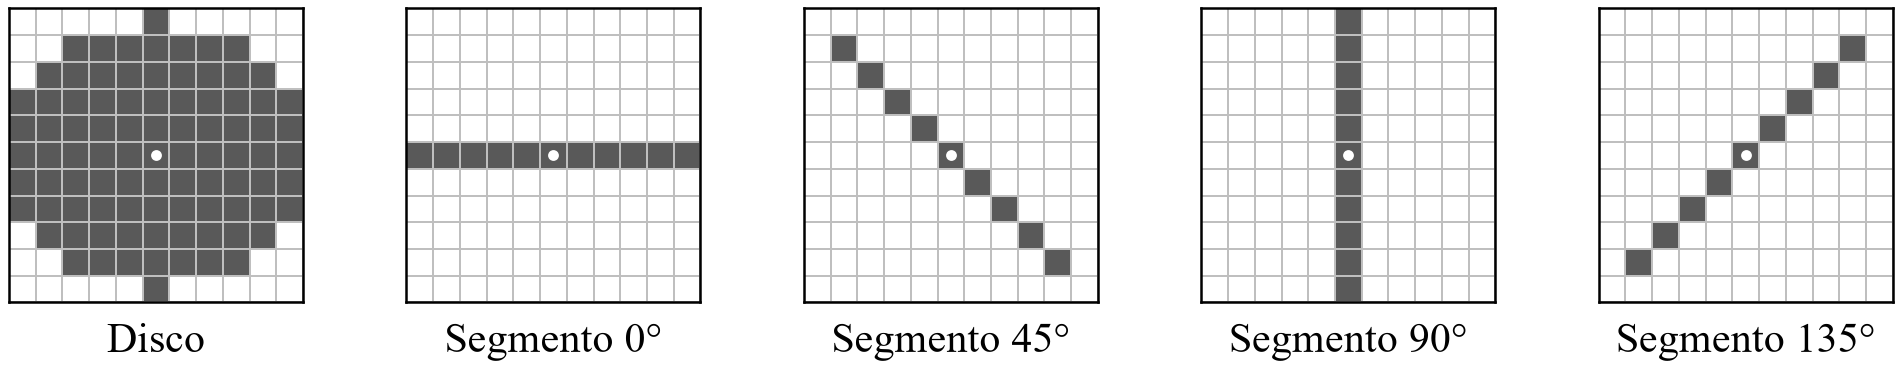
\includegraphics[width=\textwidth]{figuras/fig_banco_se}
\nota{Elaboración propia. Cada cuadro es un píxel; los cuadros grises forman el elemento, y el punto
blanco marca su centro. Con $r = 5$, cada cuadrícula mide $11 \times 11$ píxeles, y los segmentos
diagonales tienen 9 píxeles en lugar de 11. Con la configuración adoptada, $r = 25$, cada elemento ocupa
una cuadrícula de $51 \times 51$ píxeles. El disco termina en un solo píxel arriba y abajo, y no a los
costados, porque la Ecuación~\eqref{eq:disco} lo arma fila por fila y redondea el ancho de cada una.}
\end{figure}

\subsection{Combinación de las respuestas}

Con cada elemento del banco se calculan las dos transformadas de la Ecuación~\eqref{eq:wth-bth}: la
blanca, que recoge los detalles claros, y la negra, que recoge los oscuros. Como se vio en la
Sección~\ref{sec:morfologia}, el disco no distingue orientaciones, mientras que cada segmento deja en el
fondo las estructuras alineadas con él. Una estructura larga y angosta, como un poste o un cable, queda
entonces en el fondo con el segmento paralelo a ella y pasa al detalle con los otros tres. De ahí las
cuatro orientaciones: promediar sus respuestas evita que el resultado dependa de una sola dirección.

Las respuestas de los cuatro segmentos se promedian, y ese promedio se suma a la respuesta del disco.
Las transformadas del banco quedan así:
\begin{equation} \begin{aligned} \mathrm{WTH}_{\mathrm{banco}}(f) &= \mathrm{WTH}(f, D_r) + \frac{1}{4} \sum_{\theta} \mathrm{WTH}(f, S_{r,\theta}),\\
 \mathrm{BTH}_{\mathrm{banco}}(f) &= \mathrm{BTH}(f, D_r) + \frac{1}{4} \sum_{\theta} \mathrm{BTH}(f, S_{r,\theta}). \end{aligned} \label{eq:banco} \end{equation}
En esta ecuación, $\theta$ recorre los cuatro ángulos. El promedio pesa por igual las cuatro
direcciones y deja la parte de los segmentos en el mismo rango que la del disco. Con fuentes entre cero
y uno, cada parte queda entre cero y uno, y la suma, entre cero y dos: el doble del rango que daría un
único elemento.

La propuesta lleva estas transformadas a la regla de la Ecuación~\eqref{eq:regla-tophat}. Para la
imagen visible toma
\[
\mathrm{WTH}_{\mathrm{VIS}} = \mathrm{WTH}_{\mathrm{banco}}(I_{\mathrm{VIS}}),
\]
y define del mismo modo las otras tres. El resto de la regla, con su imagen base, sus máximos píxel a
píxel y su recorte, no cambia.

La Figura~\ref{fig:flujo_propuesta} reúne el algoritmo completo en un diagrama de bloques, desde las dos
imágenes de entrada hasta la imagen fusionada. Cada imagen pasa por separado por el banco, y los
detalles de las dos se combinan después con la regla y el peso $m$.

\begin{figure}[htbp]
\centering
\caption{Diagrama de bloques del algoritmo propuesto}
\label{fig:flujo_propuesta}
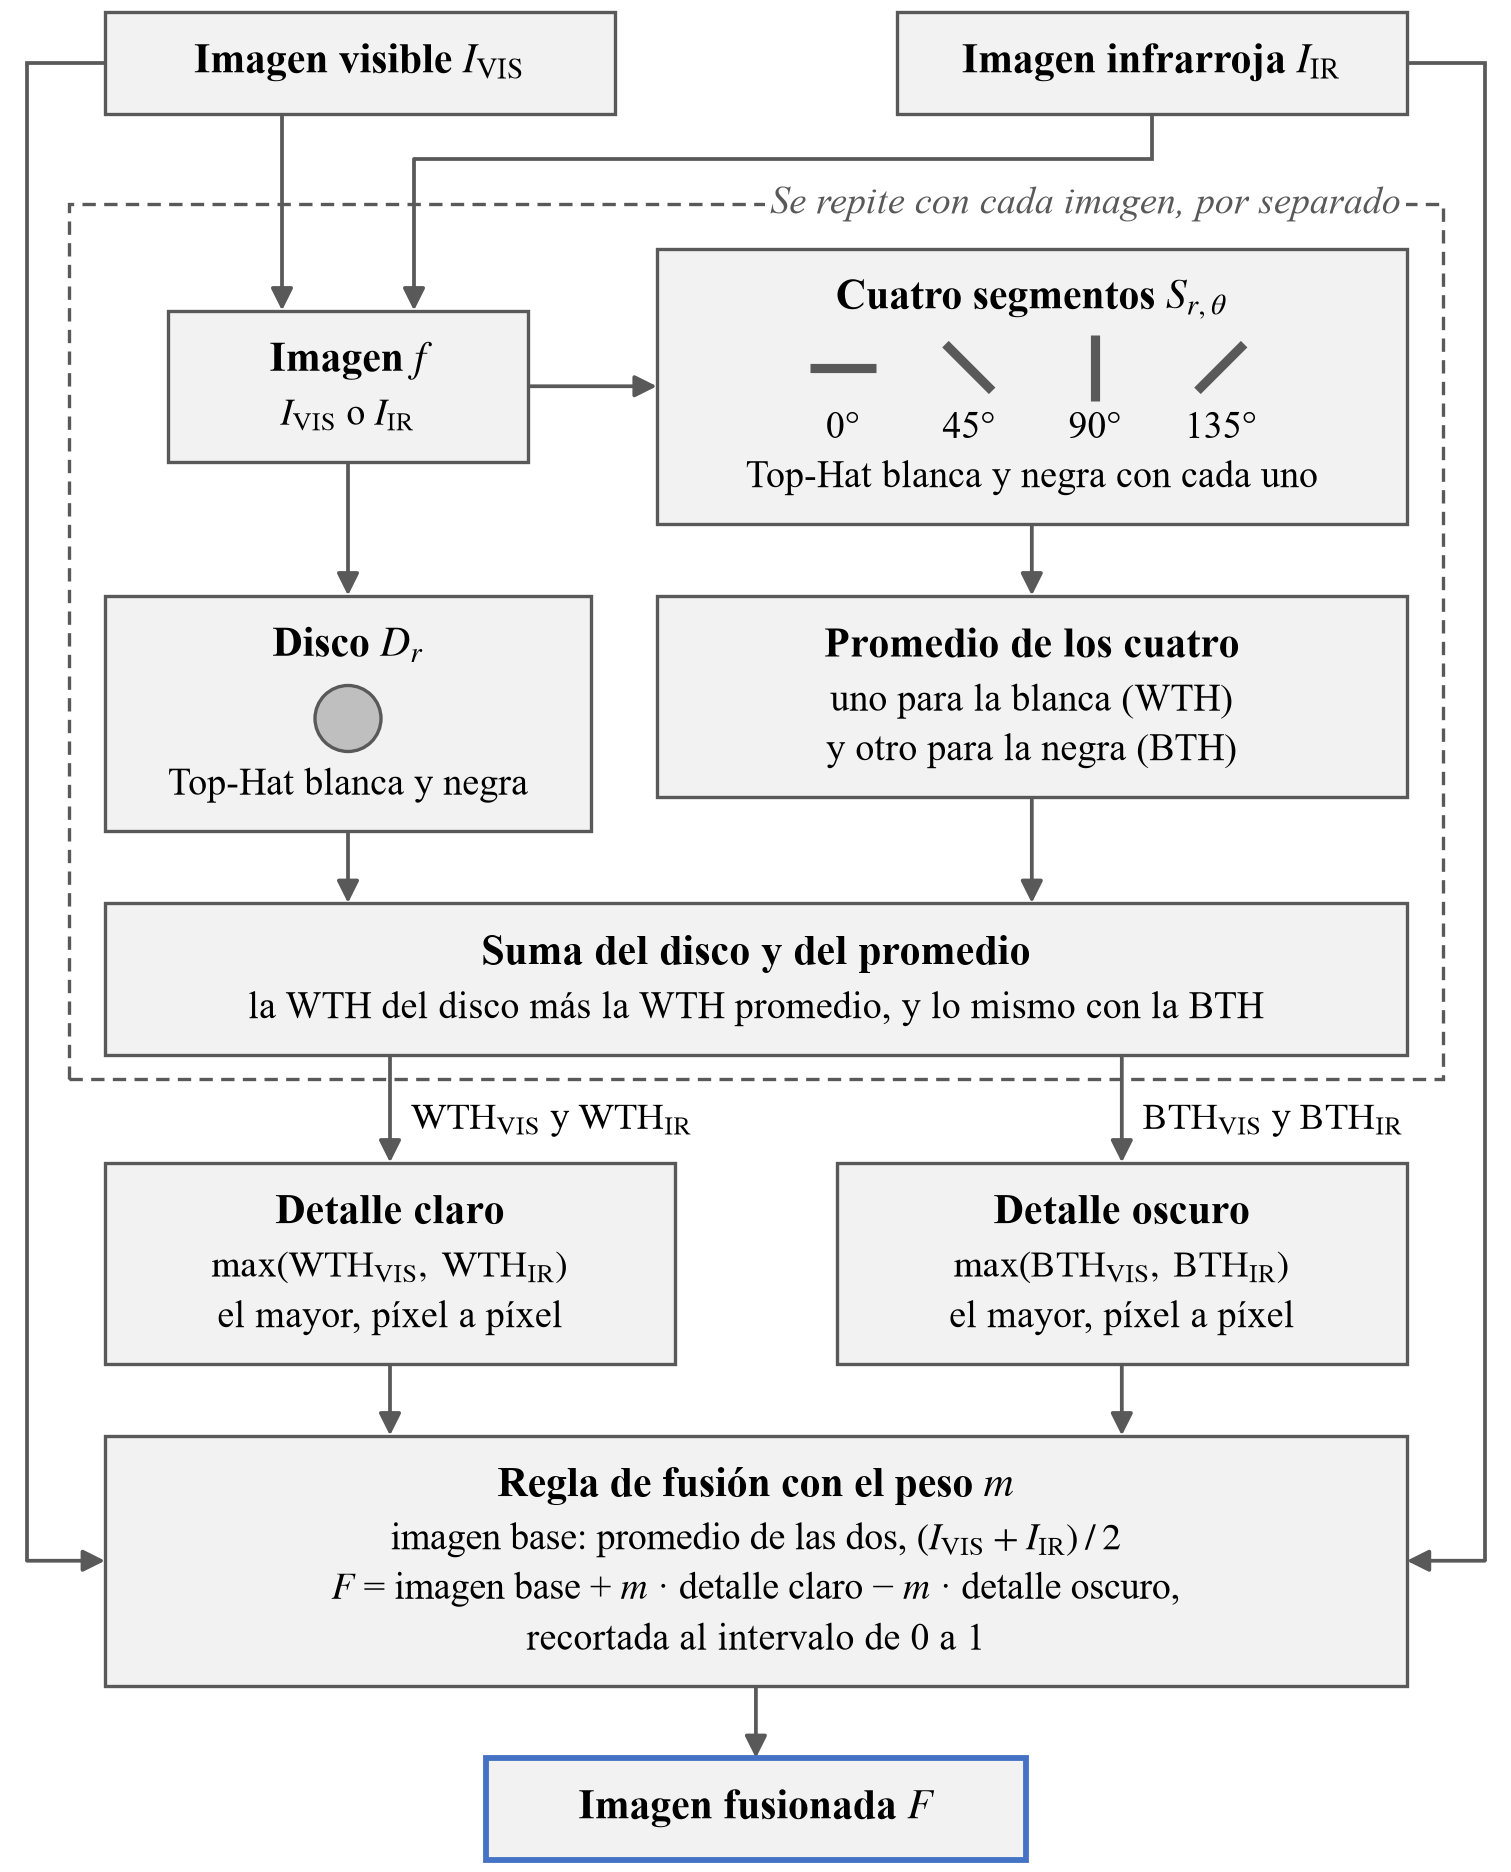
\includegraphics[width=0.8\textwidth]{figuras/fig_flujo_propuesta}
\nota{Elaboración propia. El recuadro de línea discontinua se recorre dos veces, una con la imagen
visible y otra con la infrarroja; en cada pasada, $f$ es la imagen que se procesa. Los elementos $D_r$
y $S_{r,\theta}$ se definen en las Ecuaciones~\eqref{eq:disco} y~\eqref{eq:segmentos}; WTH y BTH son las
transformadas de la Ecuación~\eqref{eq:wth-bth}. Las líneas de los costados llevan las dos imágenes de
entrada directamente a la imagen base, sin pasar por el recuadro. En la configuración adoptada, $r = 25$
y $m = 0.30$.}
\end{figure}

\subsection{Implementación y métodos comparativos}
\label{sec:operador}

La propuesta se comparó con seis métodos: el Top-Hat clásico, presentado en la
Sección~\ref{sec:fusion-tophat}, y los cinco multiescala de la Sección~\ref{sec:comparativos}. Sus
parámetros fueron los siguientes:
\begin{itemize}
\item \textbf{Top-Hat clásico:} Sigue la fusión con Top-Hat de \textcite{bajacfigueredo2024}, quienes
ensayaron elementos estructurantes de tamaños 3, 5, 7 y 9. Aquí se usa, sin ajuste, un único disco de
radio 5, es decir, de 11 píxeles de ancho, y la regla de la Ecuación~\eqref{eq:regla-tophat} con peso 1. Con ese peso, la regla agrega todo el detalle
extraído, como el realce clásico de la Ecuación~\eqref{eq:realce}.
\item \textbf{Pirámide de Laplace:} Cuatro niveles ($K = 4$), con la actividad suavizada en una ventana
de $5 \times 5$ píxeles que pesa más el centro.
\item \textbf{Pirámide de razón:} Cuatro niveles ($K = 4$), con las copias $G_0$ a $G_4$ y
$\eta = 10^{-6}$.
\item \textbf{DWT (Haar) y DWT (db4):} Tres niveles de descomposición.
\item \textbf{DTCWT:} Cuatro niveles de descomposición.
\end{itemize}
Los cinco métodos multiescala se usaron con esos parámetros, que son sus valores por defecto, sin
ajustarlos a este corpus. El Top-Hat clásico tampoco se ajustó. Entre la propuesta y el Top-Hat clásico
cambian a la vez los elementos estructurantes, el radio y el peso. Por eso, una diferencia entre los dos
no puede atribuirse al banco por sí solo.

Todos los métodos se implementaron en Python. La morfología y las pirámides se programaron con OpenCV
\parencite{bradski2000}; las transformadas \textit{wavelet}, con PyWavelets \parencite{lee2019}, y la
DTCWT, con el paquete dtcwt. Las métricas se calcularon con NumPy \parencite{harris2020}, SciPy
\parencite{virtanen2020} y scikit-image \parencite{vanderwalt2014}. Los siete métodos recibieron las
mismas entradas y pasaron por el mismo cálculo de métricas; ningún resultado se tomó de trabajos
publicados por otros autores.

Los experimentos se ejecutaron en una computadora portátil con un procesador Intel Core i7-13620H de 16 núcleos
lógicos, 31.7 GB de memoria y una tarjeta gráfica \mbox{NVIDIA} GeForce RTX 4050. La fusión y las métricas se
calcularon en el procesador, y el entrenamiento y la evaluación de los detectores se hicieron en la
tarjeta gráfica. Las versiones de los programas fueron Python 3.11, NumPy 1.26.4, OpenCV 4.13.0, SciPy 1.17.1,
scikit-image 0.26.0, PyWavelets 1.9.0, dtcwt 0.14.0, PyTorch 2.5.1 y Ultralytics 8.4.68.

\section{Ajuste de los parámetros por enjambre de partículas}
\label{sec:ajuste}

El algoritmo tiene dos parámetros. El radio $r$ define el tamaño de los cinco elementos y, con él, el
del detalle extraído, porque solo pasan a la Top-Hat los detalles en los que los elementos no caben. El
peso $m$ regula cuánto de ese detalle se suma a la imagen base. Las transformadas no dependen de $m$:
el peso solo escala el detalle antes del recorte.

Para ajustarlos se eligió la optimización por enjambre de partículas (Sección~\ref{sec:pso}), porque
es el método con que \textcite{ortegarodriguez2025} ajustan la fusión Top-Hat visible-infrarroja. De
esa obra se adaptó la función de aptitud y se tomó el rango de búsqueda: el radio
entre 1 y 25 píxeles y el peso entre 0.30 y 2.00. Las posiciones iniciales se sortearon de manera
uniforme en ese rango, y las que salían de él durante la búsqueda se llevaron al borde. Los coeficientes de la
Ecuación~\eqref{eq:pso-velocidad} valieron $c_1 = c_2 = 1.5$. La inercia bajó en línea recta, según la
Ecuación~\eqref{eq:pso-inercia}, de $w_{\max} = 0.9$ en la primera iteración a $w_{\min} = 0.4$ en la
última. La obra de referencia también usa una inercia decreciente, pero no publica sus extremos ni los
coeficientes.

La aptitud adapta la función que esa obra llama $F_o$. El radio de cada partícula se redondea al entero
más cercano, porque los elementos se arman con un número entero de píxeles. Con el radio y el peso se
fusionan los $N$ pares del ajuste, y $F_n$ es la imagen que resulta del par $n$. La aptitud es
\begin{equation} \begin{aligned} \mathrm{Apt}(r, m) = \frac{1}{N}\sum_{n=1}^{N}\biggl[ & \frac{\mathrm{SSIM}(I_{\mathrm{VIS},n}, F_n) + \mathrm{SSIM}(I_{\mathrm{IR},n}, F_n)}{2} \\
 & + \frac{\mathrm{EN}(F_n)}{8} + \frac{\mathrm{PSNR}(F_n)}{100}\biggr]. \end{aligned} \label{eq:aptitud} \end{equation}

El primer término es la similitud estructural media con las dos fuentes. A diferencia de la métrica de
la Ecuación~\eqref{eq:met-ssim}, usa la ventana que proponen \textcite{wang2004}. Esa ventana mide
$11 \times 11$ píxeles, ponderados con una curva gaussiana de desviación estándar 1.5, y el índice se
promedia sobre todas las posiciones de la imagen. El segundo término es la entropía de la
Ecuación~\eqref{eq:met-en} dividida por 8, su máximo. El tercero es la PSNR de la
Ecuación~\eqref{eq:met-psnr} dividida por 100. De los tres términos, dos premian el parecido con las
fuentes y solo la entropía premia la información de la imagen.

La obra de referencia ajusta los parámetros escena por escena. Aquí, en cambio, se buscó una sola
configuración, con la aptitud evaluada sobre tres escenas: dos con vehículos blindados y una con un
soldado detrás de una cortina de humo. De cada escena se tomó un par, y los tres pares forman parte de
los veinte con que se evaluó la calidad. El ajuste comprendió estos ensayos:
\begin{itemize}
\item \textbf{Configuraciones del enjambre:} Veinticinco corridas que, como en la obra de referencia,
cruzan cinco cantidades de partículas (2, 4, 6, 8 y 10) con cinco de iteraciones (10, 20, 30, 40 y 50).
\item \textbf{Repeticiones:} Como control de la variación al azar, las veinticinco configuraciones se
repitieron veinte veces, lo que da quinientas corridas en total.
\item \textbf{Grilla:} La aptitud se calculó en cinco mil combinaciones, que cruzan los veinticinco
radios con doscientos pesos de 0.01 a 2.00. La grilla incluye pesos menores que 0.30, fuera del rango
de búsqueda.
\item \textbf{Barrido del peso:} En las mismas tres escenas, las seis métricas se calcularon con once
pesos, de 0.05 a 2.0. El barrido abarcó la propuesta con $r = 25$ y el Top-Hat clásico con $r = 5$ y
con $r = 25$.
\end{itemize}

Como las corridas pueden terminar en radios distintos, la configuración se eligió entre los dos radios
a los que llegaron más corridas. Esos dos candidatos se compararon sobre los veinte pares del corpus
con las nueve métricas iniciales (Sección~\ref{sec:metricas}), con prioridad para las de
actividad, que reflejan el realce. La comparación usó las mismas imágenes con que después se evaluó la
calidad, una limitación que señala la Sección~\ref{sec:limitaciones}. La configuración adoptada fue
$r = 25$ y $m = 0.30$. Ese radio es uno de los dos resultados del enjambre, y se lo adoptó porque
prioriza el realce. La Sección~\ref{sec:res-ajuste} informa en qué radios y pesos terminaron las
corridas.

\section{Protocolo de evaluación de la calidad de imagen}
\label{sec:protocolo-calidad}

Como la fusión visible-infrarroja no dispone de una imagen ideal con la cual comparar el resultado, la
calidad se midió con seis métricas sin referencia, presentadas en la Sección~\ref{sec:metricas}. Tres
son de actividad y miden la información, el contraste y la nitidez de la imagen. Las otras tres son de
fidelidad y miden cuánto se parece la fusión a sus fuentes. La Tabla~\ref{tab:metricas} las resume.

\begin{table}[htbp]
\centering
\caption{Las seis métricas de evaluación de calidad}
\label{tab:metricas}
\setlength{\tabcolsep}{4pt}
\begin{tabular}{@{}lll@{}}
\toprule
\textbf{Métrica} & \textbf{Qué mide} & \textbf{Grupo} \\
\midrule
Entropía (EN)                        & cantidad de información de la imagen   & actividad \\
Desviación estándar (SD)             & contraste general                      & actividad \\
Gradiente medio (MG)                 & nitidez de los bordes                  & actividad \\
Información mutua (MI)               & cuánto de las fuentes se conserva      & fidelidad \\
Similitud estructural (SSIM)         & parecido estructural con las fuentes   & fidelidad \\
Relación señal-ruido de pico (PSNR)  & fidelidad numérica a las fuentes       & fidelidad \\
\bottomrule
\end{tabular}
\nota{Elaboración propia. Las métricas de actividad se calculan solo con la imagen fusionada, y las de
fidelidad la comparan con sus fuentes.}
\end{table}

Las seis surgen de depurar una batería inicial de nueve con dos criterios: no repetir información y
equilibrar los dos grupos. De esas nueve, las de actividad eran EN, SD, FE, MG y SF, y las de
fidelidad, la MI con cada fuente, la SSIM y la PSNR. Como comprobación, la
clasificación se repitió con esas nueve y con diecisiete: las mismas más las ocho métricas
complementarias de la Sección~\ref{sec:metricas}.

Equilibrar los grupos no impide que el ruido reciba premio, porque el ruido también eleva la actividad
de una imagen. Para medir ese efecto se agregó un control con el promedio simple y versiones degradadas
de él:
\begin{itemize}
\item \textbf{Promedio simple:} La media píxel a píxel de la visible y la infrarroja, sin detalle
agregado.
\item \textbf{Promedio con ruido:} El promedio simple con ruido gaussiano de desviación estándar 0.02,
0.05, 0.10 y 0.20.
\item \textbf{Promedio desenfocado:} El promedio simple suavizado con núcleos gaussianos de
$5 \times 5$ y de $11 \times 11$ píxeles.
\end{itemize}
Esas siete versiones de cada par se ordenaron junto con los siete métodos de fusión, con las mismas seis
métricas. Si una imagen con ruido sube en la clasificación, una actividad alta no basta para probar que
el detalle agregado sea útil.

El análisis estadístico fue no paramétrico. Con veinte pares no podía suponerse que las métricas
siguieran una distribución normal, y lo que interesaba era el orden entre los métodos. Para cada métrica
se aplicó primero la prueba de Friedman \parencite{friedman1937}, con cada par de imágenes como bloque.
Cuando resultó significativa, se aplicó la prueba de Wilcoxon de rangos con signo
\parencite{wilcoxon1945} a once contrastes entre pares de métodos. La propuesta se enfrentó con el
Top-Hat clásico y con cada uno de los cinco multiescala, y el Top-Hat clásico, con esos mismos cinco.
Los valores de $p$ se corrigieron con el procedimiento de Holm \parencite{holm1979} dentro de cada
métrica.

Cada contraste se resumió en uno de tres desenlaces. Si el valor de $p$ corregido era menor que 0.05,
contaba como victoria o como derrota, según el signo de la diferencia de medias entre los dos métodos.
Si no lo era, contaba como empate. Con seis métricas, el análisis reúne sesenta y seis decisiones de
este tipo.

Para resumir el desempeño se usó la clasificación por rango promedio. Dentro de cada par se ordenaron
los siete métodos según cada métrica, con el rango medio en caso de empate. Esos puestos se promediaron
luego sobre los pares y las métricas, y un valor más bajo indica un método mejor ubicado. El
procedimiento respeta la estructura en bloques del experimento y evita promediar magnitudes de unidades
distintas. El cálculo se repitió por separado con las métricas de actividad y con las de fidelidad, lo
que da el perfil de cada método. El rango promedio no tiene una prueba propia y se lee de forma
descriptiva.

Las pruebas tratan los veinte pares como bloques independientes, pero once de ellos provienen de solo
cuatro escenas. Para ver si esa dependencia alteraba las conclusiones, el análisis completo se repitió
con trece bloques, uno por escena. En cada escena con varias tomas, las métricas se promediaron sobre
ellas.

La evaluación se completó con una comparación visual de dos escenas, que es solo ilustrativa. Se las
eligió porque muestran dos maneras distintas en que las cámaras se complementan. En la primera, una
persona apenas se distingue en la imagen visible nocturna. En la segunda, una cortina de humo le oculta
la escena a la cámara visible. Esta segunda escena es una de las tres que se usaron en el ajuste de los
parámetros.

\section{Aplicación a la detección de objetos}
\label{sec:protocolo-deteccion}

En la aplicación que se estudia, la imagen fusionada alimenta un detector automático de objetos. La
pregunta es si, con ella, el detector encuentra lo que cada cámara ve por separado. Como un detector
aprende la apariencia de sus imágenes de entrenamiento, se entrenaron detectores propios para cada tipo
de imagen, según la práctica de \textcite{liu2022}, descrita en la Sección~\ref{sec:marco-deteccion}. Hubo diez
entradas: la visible, la infrarroja, el promedio simple y las siete fusiones. Todas usaron los mismos cuadros, las mismas
etiquetas y la misma configuración del detector.

\subsection{Partición de los datos}
\label{sec:det-datos}

Las imágenes de M3FD son cuadros de secuencias de video, y los cuadros vecinos se parecen mucho entre
sí. Si un cuadro de prueba tuviera un vecino casi idéntico en el entrenamiento, el detector se evaluaría
sobre algo que ya vio. Para evitarlo, los cuadros se agruparon en bloques de cien números de cuadro
consecutivos, y los bloques se cortaron también donde cambia el tamaño de la imagen. Los bloques,
enteros, se sortearon hasta reunir cerca del 25~\% de los cuadros para la prueba y del 10~\% para la
validación, y el resto fue al entrenamiento. Se tomó el primer sorteo que dejaba en la prueba entre el
20 y el 35~\% de las personas y de las luces. Donde se tocaban bloques de partes distintas, se
descartaron diez cuadros a cada lado del límite, 496 en total.

De los bloques de entrenamiento se tomaron al azar 2000 cuadros para entrenar. Los 474 restantes, que
aquí se llaman cuadros de seguimiento, se reservaron para seguir el entrenamiento y calibrar el umbral
de confianza. Los bloques de validación no intervinieron en el entrenamiento ni en ninguna elección, y
se sumaron a la prueba. Sobre la prueba se aplicaron luego dos filtros:
\begin{itemize}
\item \textbf{Casi duplicados en la visible:} En la imagen visible, cada cuadro se comparó con los de
entrenamiento mediante la similitud estructural. Se lo descartó si con alguno alcanzaba la mediana de
esa similitud entre cuadros consecutivos. Este filtro sacó 33 cuadros, todos de los bloques de prueba, y
dejó 1197.
\item \textbf{Parecido en las dos cámaras:} Cada cuadro se comparó también con los de entrenamiento
mediante la correlación, en la visible y en la infrarroja. Se lo descartó si, con un mismo cuadro de
entrenamiento, alcanzaba en ambas a la vez el primer cuartil de esa medida entre cuadros
consecutivos. Este filtro sacó otros 130.
\end{itemize}
La prueba final quedó en 1067 cuadros, con 2045 personas y 864 luces marcadas. Sus bloques se unieron
cuando eran contiguos, y así se formaron once grupos. En la inferencia, la unidad independiente fue el
grupo y no el cuadro, porque los cuadros de un mismo tramo de video no son independientes entre sí.

\subsection{Detector y entrenamiento}
\label{sec:det-detector}

El detector fue YOLOv8 \parencite{jocher2023} en su variante más pequeña, YOLOv8n, con la biblioteca
Ultralytics 8.4.68. Cada detector partió de los pesos con que se distribuye la red YOLOv8n,
entrenados sobre las fotografías comunes del conjunto de \textcite{lin2014}. Se lo entrenó con las seis
clases de M3FD y los 2000 cuadros de entrenamiento durante cuarenta épocas, es decir, cuarenta pasadas
completas por esos cuadros. Las imágenes se procesaron a 640 píxeles de lado, en lotes de dieciséis.
Los pesos de la red se actualizaron con el algoritmo AdamW \parencite{loshchilov2019}, con una tasa de
aprendizaje de 0.001 y un momento de 0.9. El detector se evaluó tal como quedó al final, sin elegir
ninguna época intermedia.

Para cada entrada se entrenaron tres detectores, con tres semillas distintas, y se obtuvieron así
treinta en total. La semilla fija las elecciones aleatorias del entrenamiento, entre ellas el orden de
las imágenes en los lotes y las transformaciones que se les aplican al azar. Cambiarla introduce, por lo
tanto, una variación ajena al método de fusión, que la repetición del entrenamiento permite estimar. Los detectores de la visible y
de la infrarroja se entrenaron con semillas propias, distintas de las que usaron el promedio simple y las
siete fusiones. Solo el primero de los tres entrenamientos de cada entrada se siguió época por época,
con la mAP50 sobre los cuadros de seguimiento.

\subsection{Objetos de una sola cámara y tasa de acierto equilibrada}
\label{sec:det-medida}

De las seis clases, el análisis se centró en las personas y las luces, porque su visibilidad en las dos
cámaras es opuesta. Una persona se destaca en la imagen térmica aunque esté a oscuras; una luz
encendida, en la visible. Los detectores entrenados con cada cámara lo reflejan en los 1197 cuadros que
dejó el primer filtro. En personas, la precisión media AP50 fue de 0.697 con la infrarroja y de 0.431
con la visible. En luces fue de 0.124 con la visible y de 0.020 con la infrarroja. Entre las seis
clases, la de personas es la que muestra la mayor ventaja de la infrarroja sobre la visible, y la de
luces, la mayor ventaja de la visible sobre la infrarroja.

Un objeto marcado cuenta como encontrado si el detector predice su clase con una confianza igual o
mayor que el umbral y una IoU de al menos 0.5 (Ecuación~\ref{eq:iou}). Un objeto es de una sola
cámara si lo encuentran al menos dos de los tres detectores de esa cámara y a lo sumo uno de los tres de
la otra. Si lo encuentran al menos dos de los tres detectores de cada cámara, es un objeto de las dos.

La medida principal es la tasa de acierto equilibrada. Es el promedio de dos tasas: la de acierto sobre
los objetos de solo la visible y la de acierto sobre los de solo la infrarroja. Así, ninguno de los dos
tipos de objeto pesa más por ser más numeroso. Para cada entrada, un objeto aporta la fracción de los
tres detectores de esa entrada, uno por semilla, que lo encuentran. Las tasas de la visible y de la infrarroja no
se informan, porque sus detectores son los que definen los objetos.

La confianza de cada detector tiene su propia escala, de modo que un mismo umbral no pone a todos en
igualdad de condiciones. Por eso el umbral principal se calibró detector por detector. Como referencia
se tomó la cantidad de falsos positivos de personas y luces que, en promedio, cometen por imagen los
detectores de la visible con un umbral de 0.25. A cada detector se le asignó, entre los umbrales de 0.05 a 0.95 en pasos de 0.01,
el umbral con que comete la cantidad más cercana a esa. La calibración se hizo sobre los cuadros de seguimiento, nunca sobre la prueba. Para el
análisis de sensibilidad se usaron el umbral fijo de 0.25 y el umbral de mejor equilibrio por clase. Este último
maximiza, en cada clase, la media armónica de la precisión y la exhaustividad en esos mismos cuadros.

\subsection{Comparación con el Top-Hat clásico y medidas secundarias}
\label{sec:det-comparacion}

La comparación central resta a la tasa equilibrada de la propuesta la del Top-Hat clásico, y expresa la
diferencia en puntos porcentuales. Su intervalo de confianza del 95~\% toma como unidad cada grupo de
cuadros y no cada objeto, porque los objetos de un mismo tramo de video no son independientes. Se lo
calculó con un error estándar robusto por grupos y con la distribución $t$. Sus grados de libertad
equivalen a la cantidad de grupos con objetos de una sola cámara, menos uno \parencite{cameron2015}.

Tres análisis de sensibilidad revisaron la solidez de esa diferencia:
\begin{itemize}
\item \textbf{\textit{Bootstrap} salvaje por grupos:} Se generan 9999 réplicas con la hipótesis nula
impuesta. En cada una, los residuos de cada grupo se multiplican por un peso sorteado entre seis valores
fijos, y el estadístico $t$ de la réplica se compara con el observado \parencite{cameron2008, webb2023}.
El intervalo reúne las diferencias que esta prueba no rechaza al 5~\%.
\item \textbf{Otros umbrales:} La diferencia y su intervalo se recalculan con el umbral fijo de 0.25 y
con el de mejor equilibrio por clase.
\item \textbf{Pares de semillas:} Con tres semillas por entrada hay nueve combinaciones de un detector
de la propuesta con uno del Top-Hat clásico, y cada una da su propia diferencia. La comparación se
considera robusta a la semilla si las nueve diferencias tienen el mismo signo.
\end{itemize}
Las tasas de las demás entradas, entre ellas el promedio simple y los cinco métodos multiescala, se
informan de manera descriptiva, como referencia. La diferencia entre la propuesta y el promedio simple
se calculó, además, con el mismo intervalo por grupos. Como el promedio simple es la regla de la
Ecuación~\eqref{eq:regla-tophat} con peso cero, esa diferencia estima el aporte del detalle agregado.
También se informa como referencia y no forma parte del examen de la hipótesis.

Se calcularon, además, cuatro medidas secundarias:
\begin{itemize}
\item \textbf{Precisión media global:} La mAP50 de la Ecuación~\eqref{eq:map50}, sobre las seis clases
y los 1197 cuadros que dejó el primer filtro, promediada sobre las tres semillas. Se la calculó sin
aplicar el segundo filtro, de modo que incluye los 130 cuadros que este descartó, y no interviene en el
examen de la hipótesis.
\item \textbf{Objetos de las dos cámaras:} La tasa de acierto sobre los objetos que encuentran a la vez
los detectores de la visible y los de la infrarroja.
\item \textbf{Cuadros con un objeto de cada cámara:} En los cuadros con al menos un objeto de solo la
visible y uno de solo la infrarroja, la fracción en que el detector encuentra al menos uno de cada tipo.
\item \textbf{Relación entre calidad y detección:} Para los siete métodos de fusión, la correlación de
rangos de Spearman \parencite{spearman1904} entre su rango promedio de calidad y su tasa equilibrada.
\end{itemize}
En estas medidas, las diferencias entre métodos no se sometieron a prueba.

\section{Examen de la hipótesis}
\label{sec:examen-hipotesis}

La hipótesis del trabajo, enunciada en el Capítulo~\ref{cap:introduccion}, reúne tres afirmaciones: dos
sobre la calidad de imagen y una sobre la aplicación a la detección. Cada una se examinó con las pruebas
de su evaluación, sin agregar otras:
\begin{itemize}
\item \textbf{Mejor calidad que el Top-Hat clásico:} Se usaron los seis contrastes de Wilcoxon contra
el Top-Hat clásico, uno por métrica, con la corrección de Holm. Un contraste significativo al 5~\%
contó como victoria o como derrota, según el signo de la diferencia, y uno no significativo, como
empate. El reparto se informa tal como resulta, con el rango promedio de los dos métodos como
complemento.
\item \textbf{Calidad comparable a la de los cinco métodos multiescala:} Se usaron el rango promedio con
las seis métricas y el perfil de la propuesta. El perfil reúne sus contrastes contra cada uno de los
cinco y su puesto en actividad y en fidelidad. Como el rango promedio no tiene una prueba propia y
depende de las métricas elegidas, se lo leyó junto con las clasificaciones de nueve y de diecisiete
métricas. Esta afirmación se examinó, por lo tanto, de forma descriptiva.
\item \textbf{Más objetos de una sola cámara que el Top-Hat clásico:} La afirmación se sostiene si, con
el umbral principal, el límite inferior del intervalo de confianza con la distribución $t$ supera el
cero. Se revisaron además los otros dos umbrales, el \textit{bootstrap} salvaje por grupos y los nueve
pares de semillas. Si la diferencia no resulta robusta a la semilla, se la informa como un hallazgo por
confirmar, aunque se cumpla esa condición.
\end{itemize}

En la detección, la propuesta se comparó solo con el Top-Hat clásico porque pertenece a la misma
familia y usa la misma regla de fusión (Ecuación~\ref{eq:regla-tophat}). La comparación mide, así, el
efecto de cambiar el operador en su conjunto, con sus elementos, su radio y su peso
(Sección~\ref{sec:operador}).
